\documentclass[../main.tex]{subfiles}
\graphicspath{{\subfix{images/}}}
\setlength{\parskip}{1.5em}

\begin{document}
The orbit-stabilizer theorem is a useful way to determine the order of group $G$ acting on a finite set $X$ by choosing some element $x \in X$ and by examining its orbit and stabilizer. The orbit-stabilizer theorem states that if $G$ is a group acting on a finite set $X$, then for any $x \in X$ the following must be true:
\begin{equation*}
\lvert G \rvert = \lvert Orb(x) \rvert \lvert G_x \rvert
\end{equation*}
Since this may or may not be the expected outcome I will provide an example to perhaps make this result a bit more intuitive.

\textbf{Example 1:} How many symmetries are there on a regular pentagon?

Another way of wording this question is "if you were given a pentagon, how many different orientations could you place it down in so that it occupies the same space?"

We will start off this question by numbering our pentagon, we can either number the vertices or edges but in the diagram below I have chosen to number the vertices.

\begin{center}
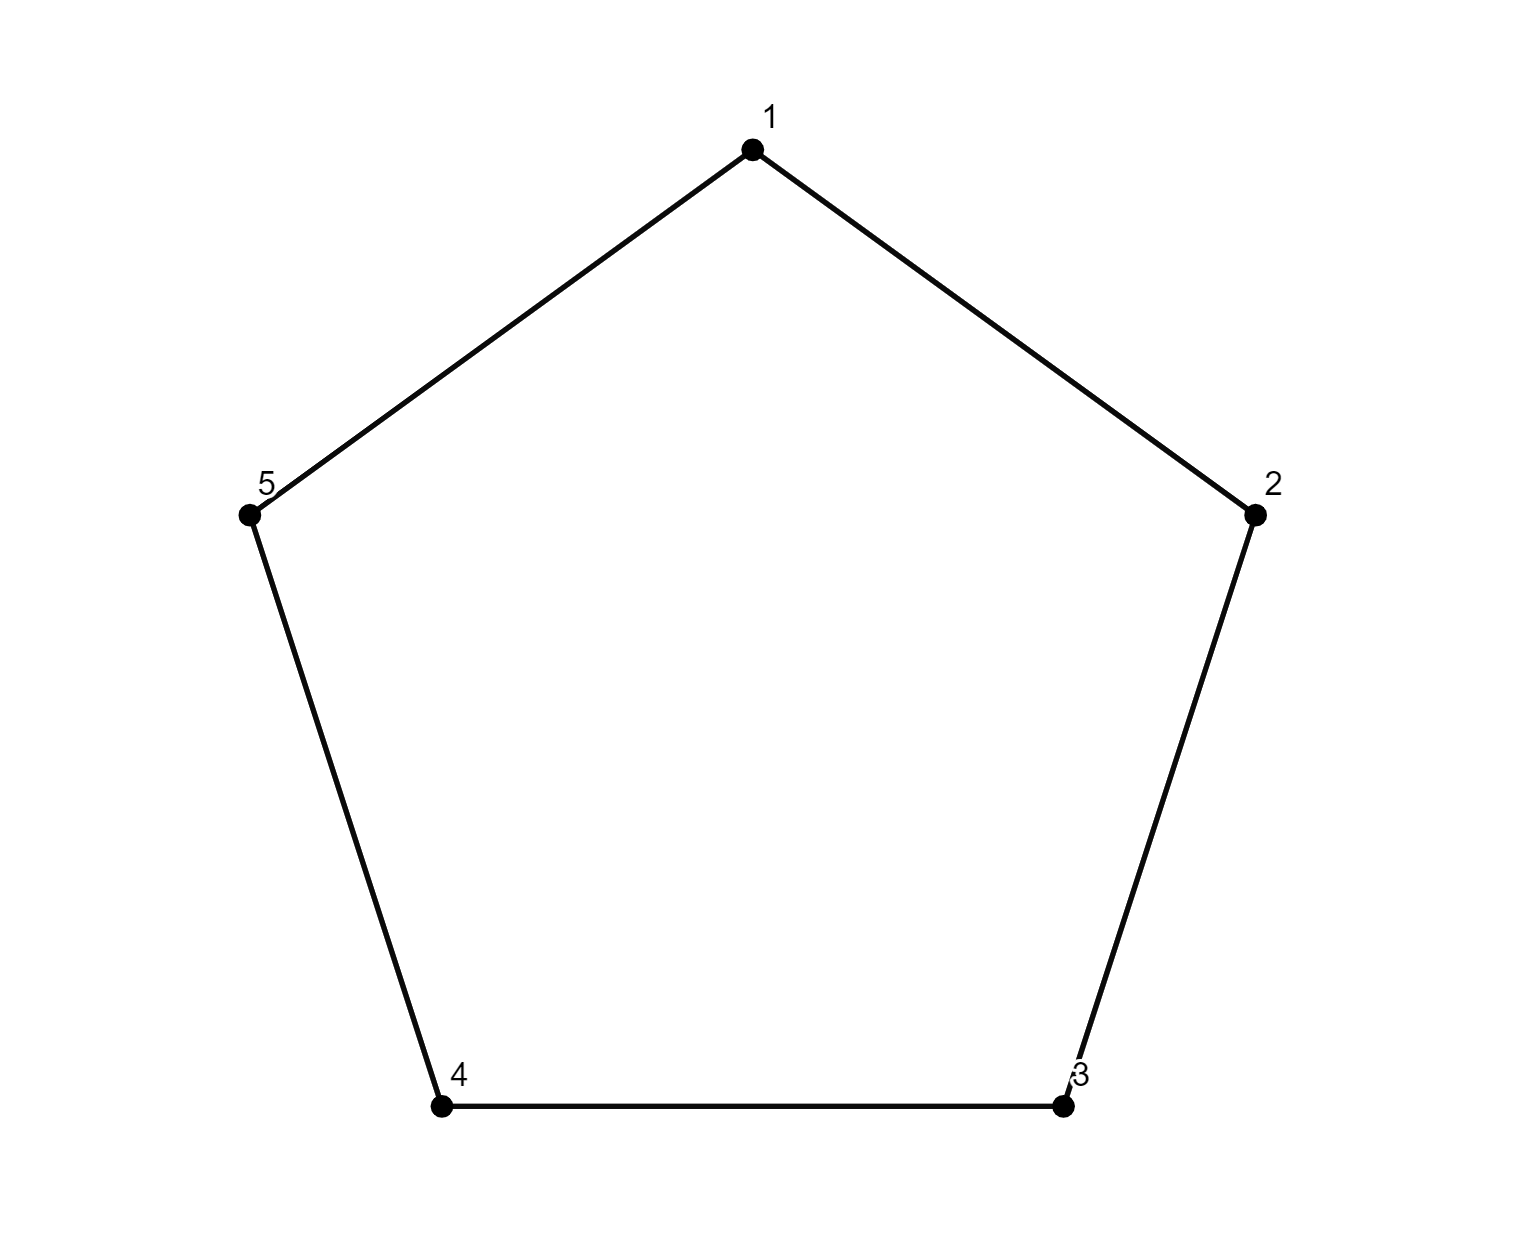
\includegraphics[width=80mm]{images/pentagon.png}
\end{center}

Now with some intuition from Gowers's \cite{gowers} we pick a vertex on the pentagon and choose where we want to place it. Note that we have 5 options for where we can place down our vertex, in this case lets choose to place our vertex  in the 1 position. Now that our vertex is fixed notice that the pentagon can still be reflected about a line through 1 and the mid point of the edge between 4 and 5, this gives us 2 possible options for each vertex for a total of $5 \cdot 2 = 10$ ways to orient the pentagon.

In this example the 5 options we get from fixing the vertex is equivalent to the orbit of $x$ and the 2 additional options on each vertex is equivalent to the stabilizer of $x$.



\end{document}
